%!TEX root = ../thesis.tex
% ******************************* Thesis Appendix F*******************************

\chapter{Wylfa Example Events In The RMon Detector}

\begin{figure}[htbp]
 \centering
 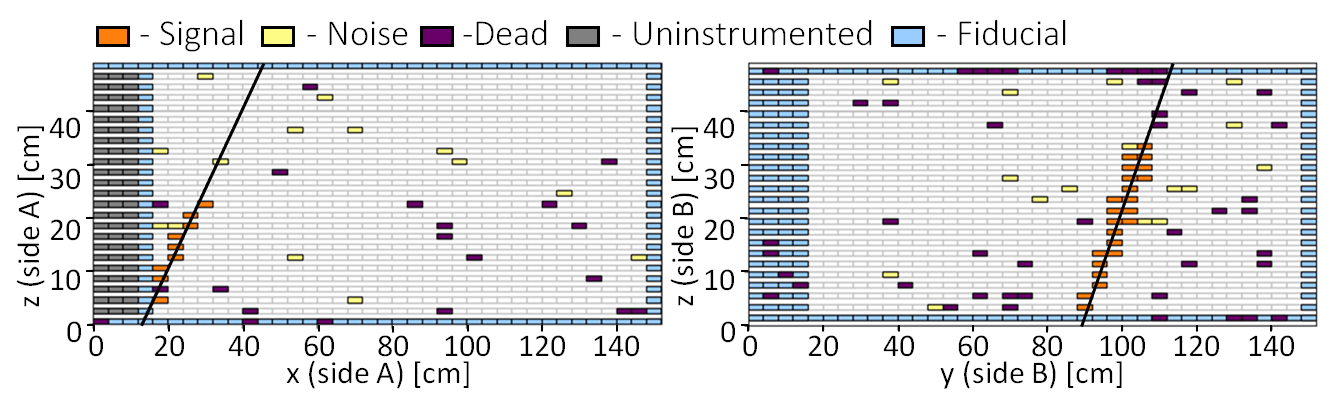
\includegraphics[width=\linewidth]{Appendix6/Figs/wylfaEg1MedText.png}
 \captionof{figure}{Example Event 1. Sometimes the electronics do not capture the whole $\mu$ track in the detector. The tracker succeeds in reconstructing these events despite the lack of a clear entry point.} 
 \label{fig:wylfaEg1}
\end{figure}

\begin{figure}[htbp]
 \centering
 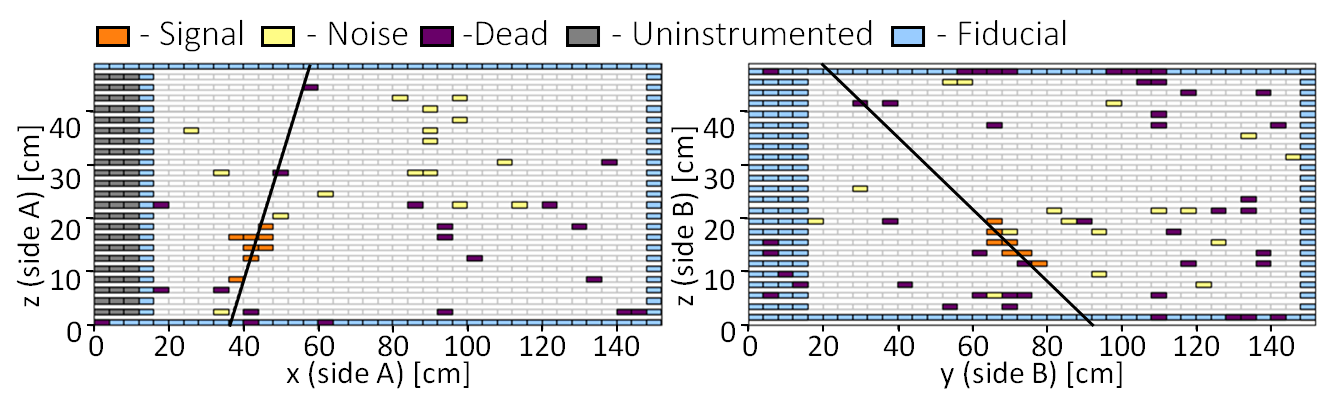
\includegraphics[width=\linewidth]{Appendix6/Figs/WylfaEg2MedText.png}
 \captionof{figure}{Example Event 2. Very Rarely most of the cosmic $\mu$ event forms a cluster, this is a consequence of the electronics an their timing. The tracker can still reconstruct these events with reasonable accuracy.} 
 \label{fig:wylfaEg2}
\end{figure}

\begin{figure}[htbp]
 \centering
 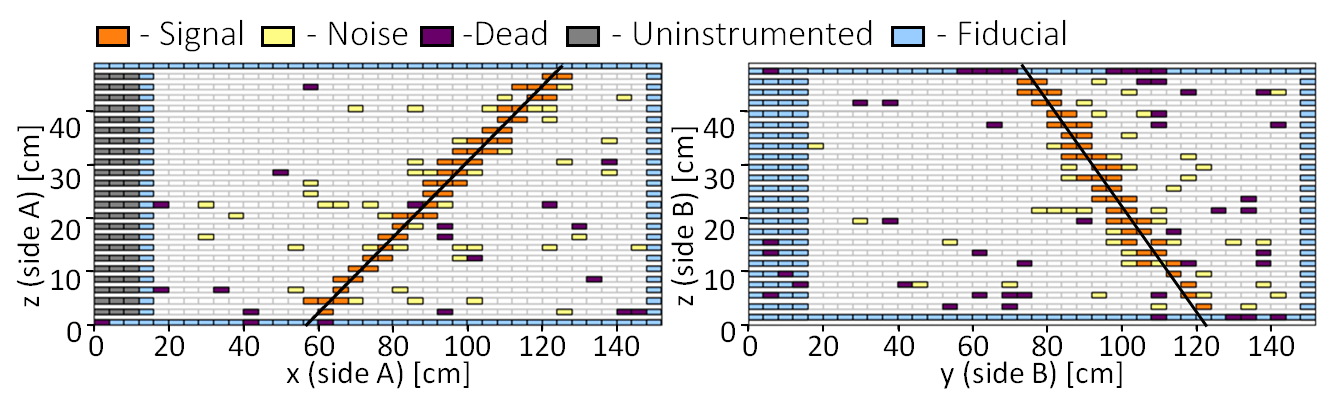
\includegraphics[width=\linewidth]{Appendix6/Figs/WylfaEg3MedText.png}
 \captionof{figure}{Example Event3. Events frequently shower in the RMon detector the high number of secondaries does not throw off the tracker and the track's reconstruction is unaffected.} 
 \label{fig:wylfaEg3}
\end{figure}

\begin{figure}[htbp]
 \centering
 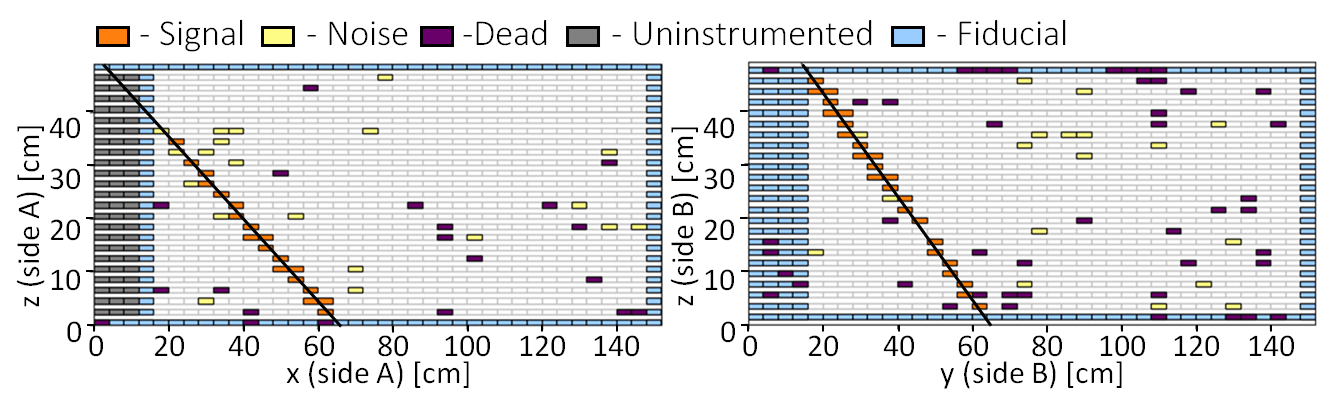
\includegraphics[width=\linewidth]{Appendix6/Figs/WylfaEg4MedText.png}
 \captionof{figure}{Example Event 4. Most of the events are large and easy to reconstruct as this one is.} 
 \label{fig:wylfaEg4}
\end{figure}

\begin{figure}[htbp]
 \centering
 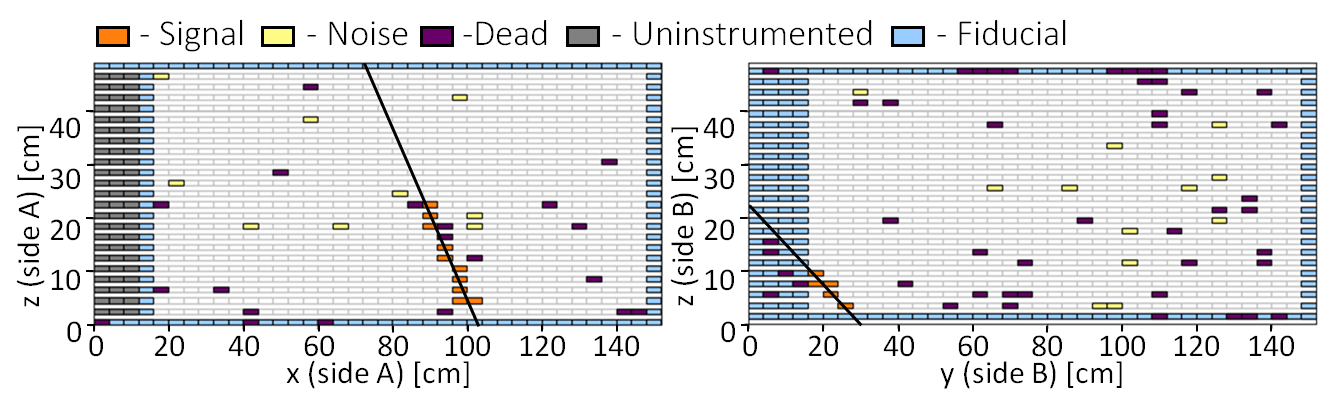
\includegraphics[width=\linewidth]{Appendix6/Figs/wylfaEg5MedText.png}
 \captionof{figure}{Example Event 5. Small corner clipping events can still be reconstructed but the uncertainty on their reconstructed $\phi$ and $\theta$ values is high.} 
 \label{fig:wylfaEg5}
\end{figure}

\begin{figure}[htbp]
 \centering
 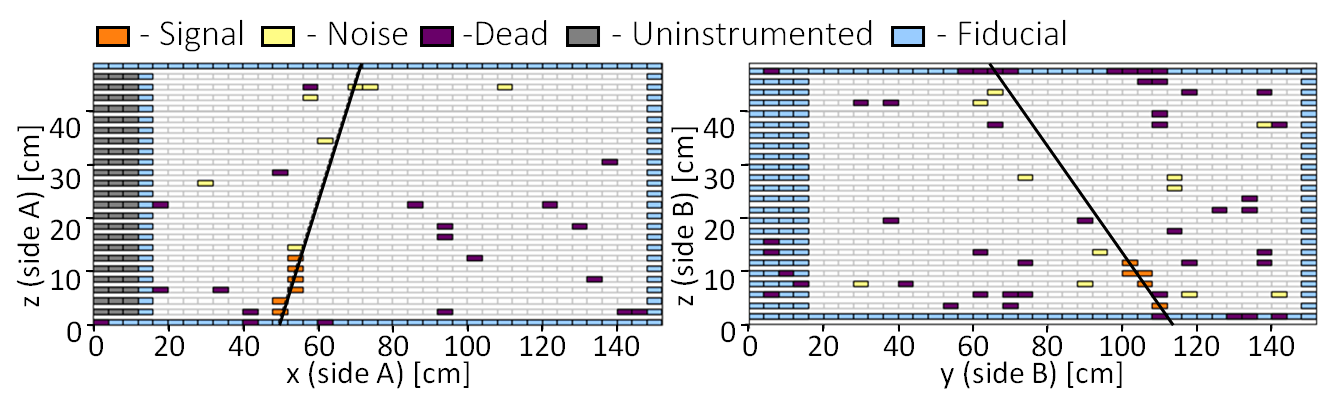
\includegraphics[width=\linewidth]{Appendix6/Figs/wylfaEg6MedText.png}
 \captionof{figure}{Example Event 6. Sometimes only a small portion of the track is visible at the bottom of the detector. The tracker can reconstruct these events but uncertainty on their reconstructed $\phi$ and $\theta$ values is high.} 
 \label{fig:wylfaEg6}
\end{figure}
